% This example is meant to be compiled with lualatex or xelatex
% The theme itself also supports pdflatex
\PassOptionsToPackage{unicode}{hyperref}
\documentclass[aspectratio=1610, xcolor=dvipsnames, 9pt]{beamer}

% Load packages you need here
\usepackage{polyglossia}
\setmainlanguage{german}

\usepackage{csquotes}
\usepackage{smartdiagram}

\usepackage{amsmath}
\usepackage{amssymb}
\usepackage{mathtools}

\usepackage{hyperref}
\usepackage{bookmark}

% load the theme after all packages

\usetheme[
  showtotalframes, % show total number of frames in the footline
]{fhswf}

% Put settings here, like
\unimathsetup{
  math-style=ISO,
  bold-style=ISO,
  nabla=upright,
  partial=upright,
  mathrm=sym,
}

\title{Explainable Artificial Intelligence}
\author[F.~Neubürger]{ \textbf{Felix Neubürger}}
\institute[I \& W]{Fachhochschule Südwestfalen, Ingenieurs- \& Wirtschaftswissenschaften}
\date{2025}
\titlegraphic{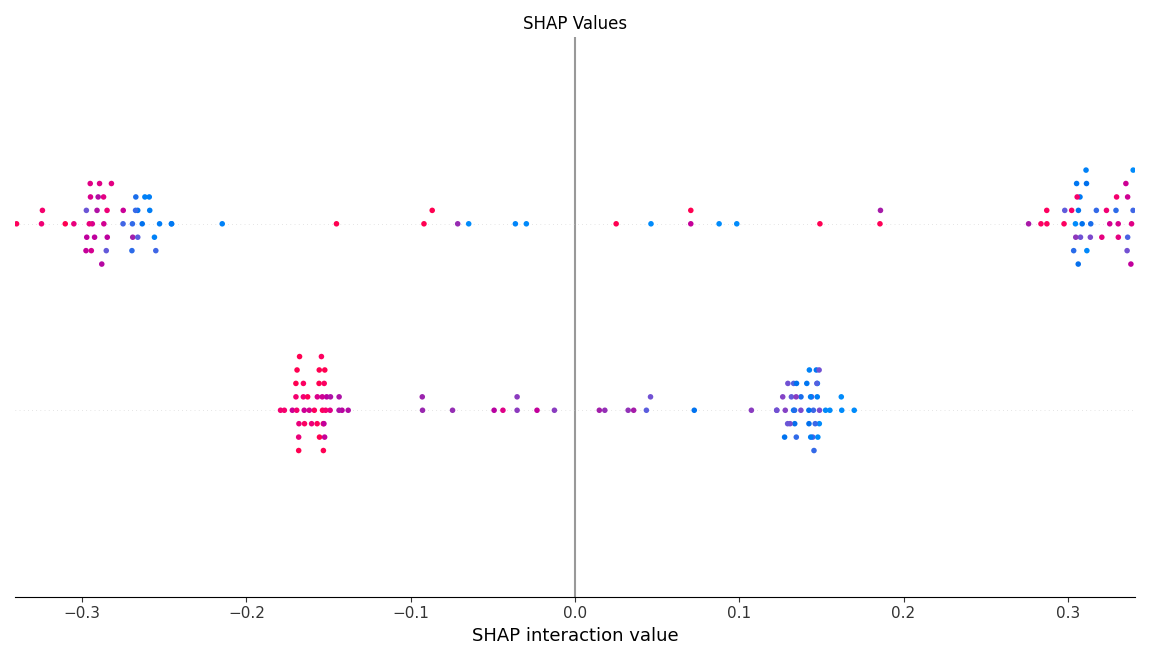
\includegraphics[width=0.6\textwidth]{images/shap_values.png}}


\begin{document}

\maketitle
\begin{frame}{Abfrage Erwartungen und Vorwissen}
  \begin{columns}
    \begin{column}{1\textwidth}
      \begin{itemize}
        \item Was verstehen Sie unter Explainable AI? \newline
        \item Haben Sie bereits Erfahrungen mit maschinellem Lernen oder KI? \newline
        \item Welche Erwartungen haben Sie an diese Vorlesung? \newline
        \item Welche Anwendungsbereiche von KI interessieren Sie besonders? \newline
        \item Gibt es spezifische Fragen, die Sie in dieser Vorlesung beantwortet haben möchten?
      \end{itemize}
    \end{column}
    \begin{column}{0\textwidth}
% \begin{figure}
% \centering
%             \includegraphics[width=0.9\textwidth]{images/intro/intro.pdf}
% \end{figure}
    \end{column}
  \end{columns}
\end{frame}

\begin{frame}{Inhalte der Vorlesung}
  \begin{columns}
    \begin{column}{1\textwidth}
      \begin{itemize}
        \item Begriffsklärungen\newline
        \item Erkenntnistheoretischer Exkurs \newline
        \item Methoden der Explainable AI  \newline
        \item Quantitative Methoden \newline 
        \item Anwendung der gelernten Methoden in einem Beispiel
      \end{itemize}
    \end{column}
    \begin{column}{0\textwidth}
% \begin{figure}
% \centering
%             \includegraphics[width=0.9\textwidth]{images/intro/intro.pdf}
% \end{figure}
    \end{column}
  \end{columns}
\end{frame}

\begin{frame}{Ziele der Vorlesung - Welche Fragen sollen beantwortet werden?}
  \begin{columns}
    \begin{column}{0.49\textwidth}
      \begin{itemize}
        \item Wofür Explainable AI? \newline
        \item Was bedeutet Explainable AI? \newline
        \item Interpretable AI?  \newline
        %\item Welche Vorteile kann Predictive Maintenance haben? \newline
        \item Trustworthy AI? \newline
        \item Wie funktioniert das mathematisch? \newline
        \item Wie schaffe ich Transparenz für Stakeholder?
        %\item Wie gehe ich an ein Predictive Maintenance Projekt heran?
      \end{itemize}
    \end{column}
    \begin{column}{0.5\textwidth}
 \begin{figure}
 \centering
             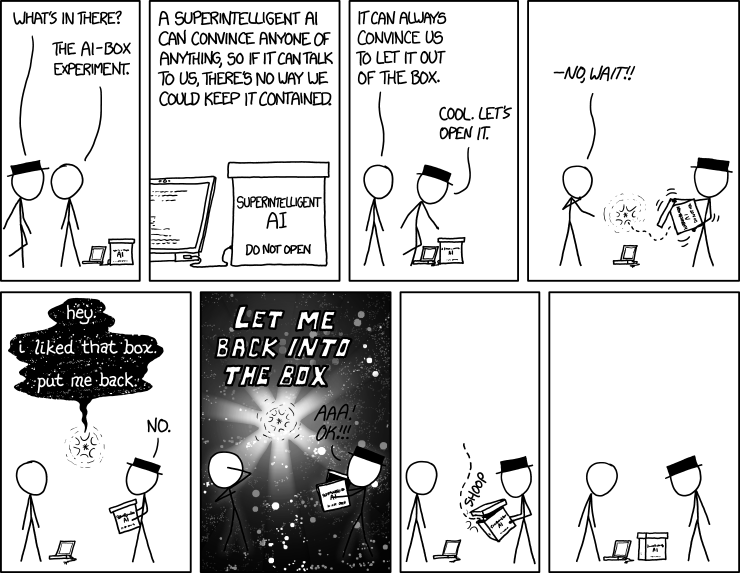
\includegraphics[width=0.9\textwidth]{images/ai_box_experiment.png}
             [\url{https://xkcd.com/1450/}]
 \end{figure}
    \end{column}
  \end{columns}
\end{frame}

\begin{frame}{Format der Vorlesung - Wie sollen diese Fragen beantwortet werden?}
  \begin{columns}
    \begin{column}{0.69\textwidth}
      \begin{itemize}
        \item Theroretischer Teil mit Folien \newline
        \item Selbststudium mt einem Lehrbuch\footnote{\url{https:// christophm.github.io/interpretable-ml-book/}} \newline
        \item Praktischer Teil in Gruppen an einem Projekt  \newline
        \item Gruppengröße 2 oder 3 Personen  \newline
        %\item Welche Vorteile kann Predictive Maintenance haben? \newline
        \item Einzelarbeit möglich wenn eigenes Thema vorhanden \newline
        \item Abgabe der Ausarbeitung einen Tag vor der Veranstaltung in der Blockwoche \newline
        \item Vorstellung der Projektergebnisse in der Blockwoche \newline
        \item Gewichtung der Bewertung Projektausarbeitung (50\%) und Vortrag (50\%)
        %
      \end{itemize}
    \end{column}
    \begin{column}{0.3\textwidth}
 \begin{figure}
 \centering
             
\includegraphics[width=0.7\textwidth]{images/tasks.png} \newline
             [\url{https://xkcd.com/1425/}]
 \end{figure}
    \end{column}
  \end{columns}
\end{frame}

\begin{frame}{Künstliche Intelligenz (KI)}
    \begin{itemize}
        \item Teilgebiet der Informatik \newline
        \item Automatisierung intelligenten Verhaltens \newline
        \item Maschinelles Lernen als Unterbereich \newline
    \end{itemize}
\end{frame}

\begin{frame}{Maschinelles Lernen (ML)}
    \begin{itemize}
        \item Unterbereich der KI \newline
        \item Algorithmen lernen aus Daten \newline
        \item Treffen von Vorhersagen oder Entscheidungen \newline
        \item Deep Learning basiert auf künstlichen neuronalen Netzen
    \end{itemize}
\end{frame}

\begin{frame}{Explainable Artificial Intelligence (XAI)}
    \begin{itemize}
        \item Ansätze zur Verständlichkeit von KI-Entscheidungen \newline
        \item Wichtig für Vertrauen und Transparenz \newline
        \item Beispiel: Erklärungen in der medizinischen Diagnostik
    \end{itemize}
\end{frame}

\begin{frame}{Definitionen und Unterschiede}
    \begin{block}{Interpretierbarkeit}
        \begin{itemize}
            \item Fähigkeit, die internen Mechanismen eines Modells zu verstehen. 
            \item Ermöglicht direkte Einsicht in die Funktionsweise des Modells.
            \item Beispiel: Lineare Regression, Entscheidungsbäume.
        \end{itemize}
    \end{block}
    \begin{block}{Erklärbarkeit}
        \begin{itemize}
            \item Fähigkeit, die Entscheidungen oder Vorhersagen eines Modells verständlich zu machen.
            \item Oft durch zusätzliche Methoden bei komplexen Modellen erreicht.
            \item Beispiel: Neuronale Netze mit Post-hoc-Erklärungen.
        \end{itemize}
    \end{block}
\end{frame}

\begin{frame}{Erkenntnistheoretische Aspekte}
    \begin{itemize}
        \item \textbf{Wissenserwerb:} Wie tragen Interpretierbarkeit und Erklärbarkeit zum Verständnis von KI-Entscheidungen bei? \newline
        \item \textbf{Vertrauen:} Inwiefern beeinflusst die Nachvollziehbarkeit von Modellen das Vertrauen der Nutzer? \newline
        \item \textbf{Transparenz vs. Komplexität:} Balance zwischen detaillierter Einsicht und praktischer Anwendbarkeit. \newline
        \item \textbf{Ethische Verantwortung:} Bedeutung von Erklärbarkeit für ethisch vertretbare KI-Systeme. 
    \end{itemize}
\end{frame}

\begin{frame}{Bedeutung der Interpretierbarkeit im Maschinellen Lernen}
    \begin{itemize}
        \item \textbf{Definition:} \newline
        Interpretierbarkeit bezeichnet das Maß, in dem ein Mensch die Ursache einer Entscheidung eines Modells nachvollziehen kann.
        \newline
        \item \textbf{Warum ist Interpretierbarkeit wichtig?}
        \begin{itemize}
            \item \textbf{Vertrauensbildung:} \newline
            Nutzer vertrauen eher Modellen, deren Entscheidungswege sie verstehen.
            \item \textbf{Fehleranalyse:} \newline
            Verständnis für Modellentscheidungen erleichtert das Erkennen und Beheben von Fehlern.
            \item \textbf{Einhaltung gesetzlicher Vorgaben:} \newline
            In sensiblen Bereichen wie Medizin oder Finanzen sind nachvollziehbare Entscheidungen oft gesetzlich vorgeschrieben.
        \end{itemize}
    \end{itemize}
\end{frame}

\begin{frame}{Herausforderungen und Begriffsabgrenzungen}
    \begin{itemize}
        \item \textbf{Herausforderungen:}
        \begin{itemize}
            \item Fehlende einheitliche Definition von Interpretierbarkeit erschwert Kommunikation und Forschung.
            \item Kompromiss zwischen Modellkomplexität und Interpretierbarkeit oft notwendig.
        \end{itemize}
        \item \textbf{Abgrenzung zu verwandten Begriffen:}
        \begin{itemize}
            \item \textbf{Erklärbarkeit (Explainability):} \newline
            Fähigkeit, interne Mechanismen eines Modells verständlich zu machen.
            \item \textbf{Transparenz:} \newline
            Ausmaß, in dem die Funktionsweise eines Modells offenliegt.
            \item \textbf{Vertrauen:} \newline
            Maß, in dem Nutzer darauf vertrauen, dass ein Modell korrekte und faire Entscheidungen trifft.
        \end{itemize}
    \end{itemize}
\end{frame}

\begin{frame}
    \frametitle{EU-Regulierung und Erklärbare Künstliche Intelligenz}
Die Europäische Union hat den Artificial Intelligence Act verabschiedet,\footnote{Regulation (EU) 2024/1689 des Europäischen Parlaments und des Rates vom 13. Juni 2024 über harmonisierte Vorschriften für künstliche Intelligenz. Verfügbar unter: \url{https://eur-lex.europa.eu/eli/reg/2024/1689/oj}} der am 1. August 2024 in Kraft trat.\footnote{Pressemitteilung der Europäischen Kommission: "AI Act tritt in Kraft". Verfügbar unter: \url{https://ec.europa.eu/commission/presscorner/detail/de/ip_24_1234}}

    \textbf{EU AI Act: Überblick}
    \begin{itemize}
        \item \textbf{Ziel:} Einführung eines risikobasierten Klassifizierungssystems für KI-Anwendungen.  \newline
        \item \textbf{Risikokategorien:}
        \begin{itemize}
            \item \textbf{Unzulässiges Risiko:} Verbotene KI-Anwendungen.
            \item \textbf{Hohes Risiko:} Strenge Anforderungen an Transparenz, Sicherheit und Compliance.
            \item \textbf{Geringes oder minimales Risiko:} Weniger strenge oder keine spezifischen Anforderungen.
        \end{itemize}
    \end{itemize}

    \textbf{Erklärbarkeit als zentrale Anforderung} \newline
    \begin{itemize}
        \item \textbf{Transparenzpflichten:} Anbieter müssen Informationen bereitstellen, die es ermöglichen, die Funktionsweise von KI-Systemen zu verstehen.
        \item \textbf{Vertrauenswürdigkeit:} Erklärbare KI fördert das Vertrauen der Nutzer und erleichtert die Akzeptanz von KI-Technologien.
    \end{itemize}

\end{frame}

\begin{frame}
    \frametitle{Herausforderungen des EU AI Acts für Unternehmen}

    \begin{itemize}
        \item \textbf{Komplexität der Regulierung:} \\
        Der AI Act verfolgt einen risikobasierten Ansatz, bei dem KI-Systeme in verschiedene Risikoklassen eingeteilt werden. Unternehmen müssen ihre KI-Anwendungen entsprechend einstufen und die jeweiligen Anforderungen erfüllen.\footnote{\url{https://www.it-schulungen.com/wir-ueber-uns/wissensblog/welche-anforderungen-stellt-der-eu-ai-act.html}}

        \item \textbf{Standardisierung und technische Umsetzung:} \\
        Die Entwicklung harmonisierter Standards für Hochrisiko-KI-Systeme ist komplex und zeitaufwendig. Verzögerungen können zu Unsicherheiten bei der Implementierung führen und Innovationen hemmen.\footnote{\url{https://www.connect-professional.de/security/der-ai-act-chancen-nutzen-risiken-managen.332959.html}}

        \item \textbf{Vermeidung von Innovationshemmnissen:} \\
        Es besteht die Sorge, dass strenge Regulierungen Innovationen im Bereich der Künstlichen Intelligenz behindern könnten. Unternehmen müssen Wege finden, um sowohl den gesetzlichen Anforderungen zu entsprechen als auch ihre Innovationsfähigkeit zu bewahren.\footnote{\url{https://www.dps-bs.de/blog/der-ai-act-weichenstellung-fuer-kuenstliche-intelligenz-in-europa/}}

        \item \textbf{Wettbewerbsfähigkeit im internationalen Kontext:} \\
        Unternehmen in Regionen mit weniger strengen Vorschriften könnten schneller Innovationen umsetzen und dadurch Wettbewerbsvorteile erlangen. Europäische Firmen stehen vor der Herausforderung, trotz strengerer Regulierungen konkurrenzfähig zu bleiben.\footnote{\url{https://de.linkedin.com/pulse/der-eu-ai-act-chancen-und-herausforderungen-f\%C3\%BCr-andreas-quandt-ljxne}}
    \end{itemize}

\end{frame}

\begin{frame}{Methoden der Explainable AI (XAI)}
  \begin{columns}
    \begin{column}{1\textwidth}
      \textbf{Global interpretierbare Modelle:}
      \begin{itemize}
        \item Lineare Regression
        \item Entscheidungsbäume
        \item Regelbasierte Modelle
      \end{itemize}
      \vspace{0.5cm}
      \textbf{Post-hoc Erklärungen:}
      \begin{itemize}
        \item Lokale Methoden (z.B. LIME, SHAP)
        \item Visualisierungen (z.B. Feature Importance, PDPs)
        \item Gegenbeispiele (Counterfactual Explanations)
      \end{itemize}
      \vspace{0.5cm}
      \textbf{Surrogatmodelle:}
      \begin{itemize}
        \item Vereinfachte Modelle, die komplexe Modelle approximieren
      \end{itemize}
    \end{column}
    %\begin{column}{0.0\textwidth}
    %  \includegraphics[width=\textwidth]{images/xai_methods.png}
    %\end{column}
  \end{columns}
\end{frame}

\begin{frame}{Globale Methoden}
  \begin{columns}
    \begin{column}{1\textwidth}
      \textbf{Feature Importance:}
      \begin{itemize}
        \item Bewertung der Bedeutung einzelner Merkmale
      \end{itemize}
      \vspace{0.3cm}
      \textbf{Permutation Feature Importance:}
      \begin{itemize}
        \item Bewertung durch Permutation der Merkmale
      \end{itemize}
      \vspace{0.3cm}
      \textbf{Partial Dependence Plots (PDP):}
      \begin{itemize}
        \item Einfluss eines Merkmals auf die Vorhersage
      \end{itemize}
      \vspace{0.3cm}
      \textbf{Global Surrogates:}
      \begin{itemize}
        \item Erklärbares Modell, das ein komplexes Modell nachahmt
      \end{itemize}
    \end{column}
    %\begin{column}{0.4\textwidth}
    %  \includegraphics[width=\textwidth]{images/global_methods.png}
    %\end{column}
  \end{columns}
\end{frame}

\begin{frame}{Lokale Methoden}
  \begin{columns}
    \begin{column}{1\textwidth}
      \textbf{LIME:}
      \begin{itemize}
        \item Lokale lineare Approximationen des Modells
      \end{itemize}
      \vspace{0.3cm}
      \textbf{SHAP:}
      \begin{itemize}
        \item Spieltheorie-basierte Quantifizierung von Merkmalbeiträgen
      \end{itemize}
      \vspace{0.3cm}
      \textbf{Counterfactual Explanations:}
      \begin{itemize}
        \item Minimale Änderungen für eine andere Vorhersage
      \end{itemize}
    \end{column}
    %\begin{column}{0.4\textwidth}
    %  \includegraphics[width=\textwidth]{images/local_methods.png}
    %\end{column}
  \end{columns}
\end{frame}

\begin{frame}{Visualisierungen}
  \begin{columns}
    \begin{column}{1\textwidth}
      \textbf{Feature Importance:}
      \begin{itemize}
        \item Balkendiagramme zur Darstellung der Merkmalsbedeutung
      \end{itemize}
      \vspace{0.3cm}
      \textbf{Partial Dependence Plots (PDP):}
      \begin{itemize}
        \item Einfluss eines Merkmals auf die Vorhersage
      \end{itemize}
      \vspace{0.3cm}
      \textbf{Individual Conditional Expectation (ICE):}
      \begin{itemize}
        \item Individuelle Effekte von Merkmalen für einzelne Datenpunkte
      \end{itemize}
    \end{column}
    %\begin{column}{0.4\textwidth}
    %  \includegraphics[width=\textwidth]{images/visualizations.png}
    %\end{column}
  \end{columns}
\end{frame}

\begin{frame}
  \frametitle{Lineare Modelle}
  \begin{columns}
    \begin{column}{1\textwidth}
      \textbf{Lineare Regression:}
      \begin{itemize}
        \item Modell: $Y = \beta_0 + \beta_1 X_1 + \dots + \beta_p X_p + \epsilon$
        \item $\beta_0$: Achsenabschnitt
        \item $\beta_i$: Regressionskoeffizienten
        \item $\epsilon$: Fehlerterm
      \end{itemize}
      \vspace{0.5cm}
      \textbf{Generalisierte Additive Modelle (GAMs):}
      \begin{itemize}
        \item Modell: $Y = \beta_0 + f_1(X_1) + \dots + f_p(X_p) + \epsilon$
        \item $f_i$: Glatte Funktionen für nichtlineare Beziehungen
      \end{itemize}
    \end{column}
    %\begin{column}{0.4\textwidth}
    %  \includegraphics[width=\textwidth]{images/linear_models.png}
    %\end{column}
  \end{columns}
\end{frame}

\begin{frame}
  \frametitle{Entscheidungsbäume}
  \begin{columns}
    \begin{column}{0.6\textwidth}
      \begin{itemize}
        \item Rekursive Partitionierung des Merkmalsraums
        \item Jeder Knoten: Entscheidung basierend auf Merkmal und Schwellenwert
        \item Ziel: Maximierung der Homogenität in den Blättern
      \end{itemize}
    \end{column}
    \begin{column}{0.4\textwidth}
      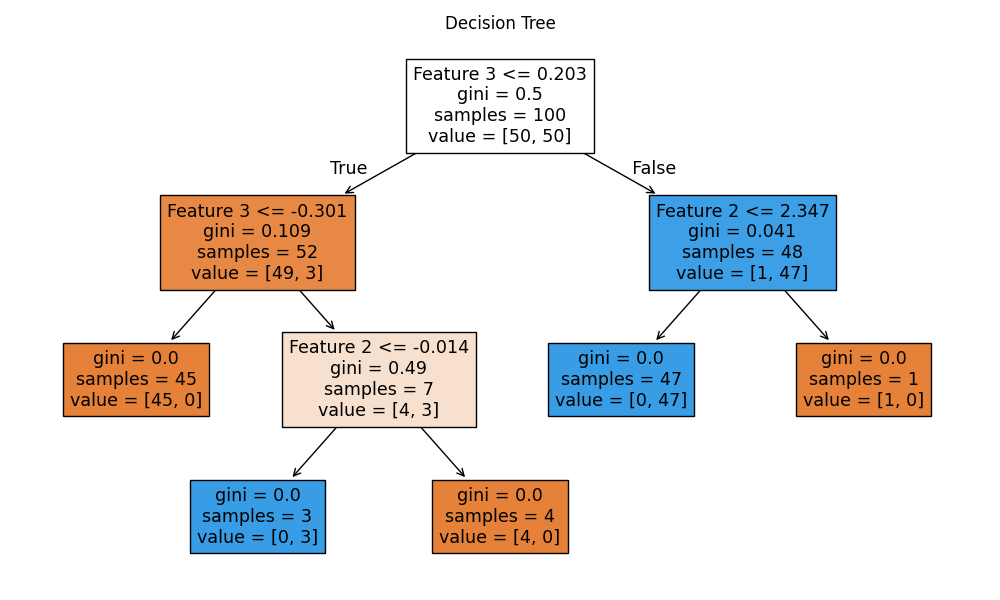
\includegraphics[width=\textwidth]{images/decision_trees.png}
    \end{column}
  \end{columns}
\end{frame}

\begin{frame}
  \frametitle{Modellagnostische Methoden}
  \begin{columns}
    \begin{column}{1\textwidth}
      \textbf{Permutation Feature Importance:}
      \begin{itemize}
        \item Permutation eines Merkmals
        \item Messung des Anstiegs des Vorhersagefehlers
        \item Signifikanter Anstieg = hohe Bedeutung
      \end{itemize}
      \vspace{0.5cm}
      \textbf{Partielle Abhängigkeitsdiagramme (PDPs):}
      \begin{itemize}
        \item Zeigen durchschnittliche Wirkung eines Merkmals
        \item Berechnung: $\hat{f}_{X_S}(x_S) = \mathbb{E}_{X_C}[\hat{f}(x_S, X_C)]$
      \end{itemize}
      \vspace{0.5cm}
      \textbf{Akkumulierte lokale Effekte (ALE):}
      \begin{itemize}
        \item Messen durchschnittliche Änderung der Vorhersage
        \item Berechnung: $ALE_j(x) = \int_{x_{min}}^x \mathbb{E} \left[ \frac{\partial \hat{f}(x)}{\partial x_j} \mid x_j = z \right] dz$
      \end{itemize}
    \end{column}
    %\begin{column}{0.4\textwidth}
    %  \includegraphics[width=\textwidth]{images/model_agnostic.png}
    %\end{column}
  \end{columns}
\end{frame}

\begin{frame}
  \frametitle{SHAP-Werte}
  \begin{columns}
    \begin{column}{0.6\textwidth}
      \begin{itemize}
        \item Basieren auf kooperativer Spieltheorie
        \item Beitrag jedes Merkmals zur Vorhersage:
        \item $\phi_i = \sum_{S \subseteq N \setminus \{i\}} \frac{|S|! (|N| - |S| - 1)!}{|N|!} \left[ f(S \cup \{i\}) - f(S) \right]$
      \end{itemize}
    \end{column}
    \begin{column}{0.4\textwidth}
      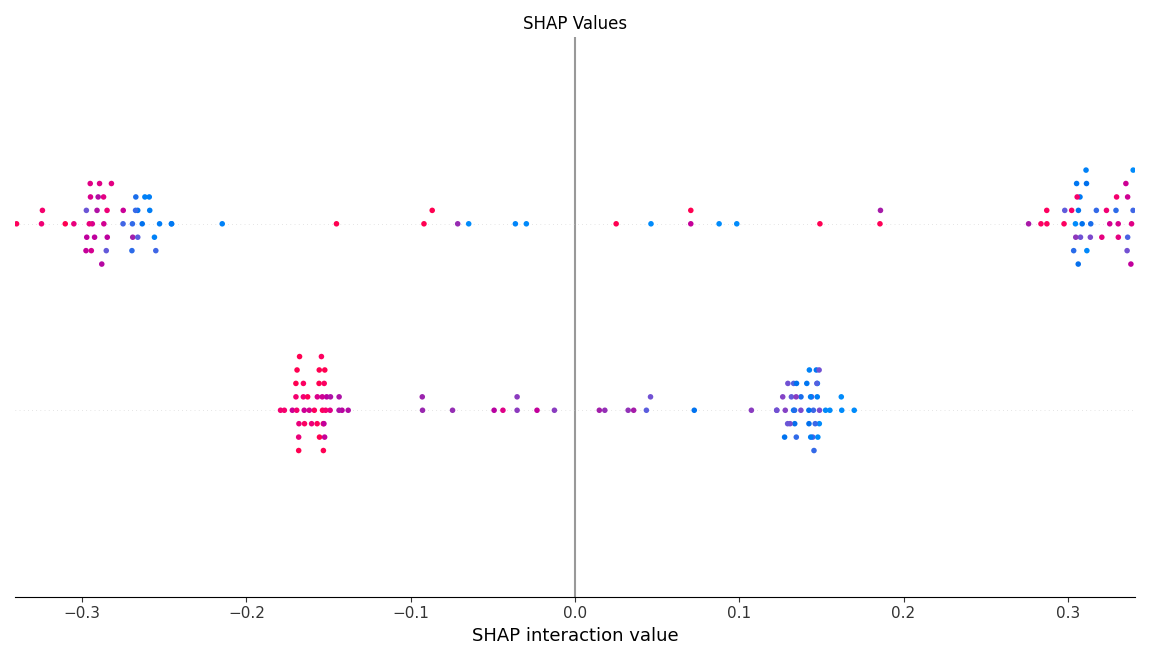
\includegraphics[width=\textwidth]{images/shap_values.png}
    \end{column}
  \end{columns}
\end{frame}

\begin{frame}
  \frametitle{Lokale Surrogatmodelle: LIME}
  \begin{columns}
    \begin{column}{0.6\textwidth}
      \begin{itemize}
        \item Einfaches Modell (z.B. lineare Regression) lokal anpassen
        \item Künstliche Datenpunkte in der Nähe generieren
        \item Gewichtung basierend auf Ähnlichkeit zur Instanz
      \end{itemize}
    \end{column}
    \begin{column}{0.4\textwidth}
      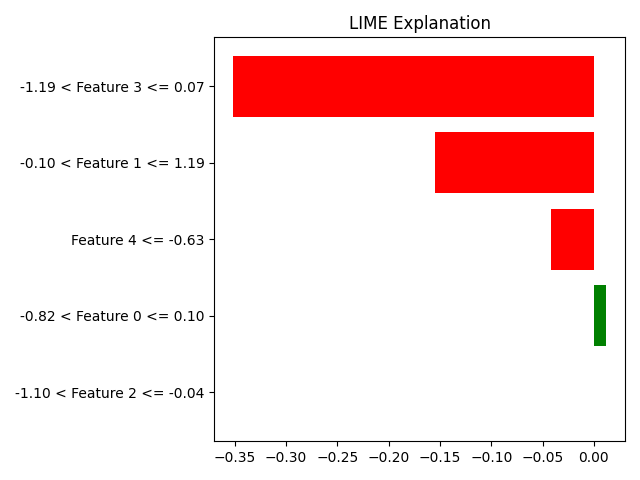
\includegraphics[width=\textwidth]{images/lime.png}
    \end{column}
  \end{columns}
\end{frame}

\begin{frame}
  \frametitle{Methoden zur Interpretation neuronaler Netzwerke}
  \begin{itemize}
      \item \textbf{Feature Visualization:}
      \begin{itemize}
          \item Visualisierung der Merkmale, auf die Neuronen reagieren.
          \item Ermöglicht Einblicke in die von Neuronen erkannten Muster.
      \end{itemize}
      \item \textbf{Saliency Maps:}
      \begin{itemize}
          \item Identifikation von Eingabebereichen, die den größten Einfluss auf die Ausgabe haben.
          \item Darstellung der Bedeutung einzelner Pixel oder Merkmale.
      \end{itemize}
      \item \textbf{Layer-wise Relevance Propagation (LRP):}
      \begin{itemize}
          \item Rückverfolgung der Entscheidung des Netzwerks auf die Eingabedaten.
          \item Zuweisung von Relevanzwerten zu einzelnen Eingabeelementen.
      \end{itemize}
  \end{itemize}
  \begin{figure}
      \centering
      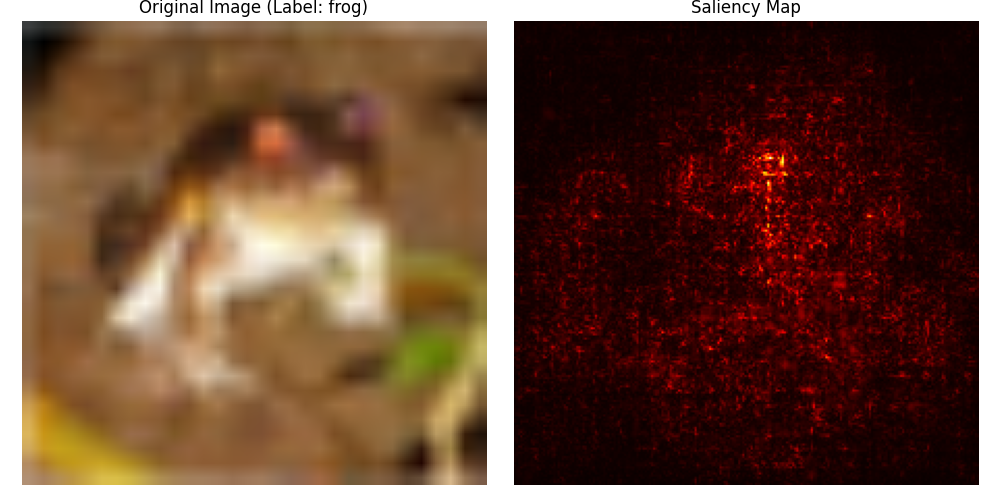
\includegraphics[width=0.5\textwidth]{images/saliency_map.png}
      \caption{Beispiel einer Saliency Map}
  \end{figure}
\end{frame}

\begin{frame}
  \frametitle{Werkzeuge und Bibliotheken für erklärbare KI}
  \begin{itemize}
      \item \textbf{Captum:}
      \begin{itemize}
          \item PyTorch-Bibliothek für Interpretierbarkeitsmethoden.
          \item Unterstützt Techniken wie integrierte Gradienten und DeepLIFT.
      \end{itemize}
      \item \textbf{ELI5:}
      \begin{itemize}
          \item Bibliothek zur Erklärung von ML-Modellen und Vorhersagen.
          \item Unterstützt verschiedene Modelle wie Sklearn, XGBoost und Keras.
      \end{itemize}
      \item \textbf{SHAP-Bibliothek:}
      \begin{itemize}
          \item Implementierung der SHAP-Werte für verschiedene Modelltypen.
          \item Ermöglicht detaillierte Analysen der Merkmalsbeiträge.
      \end{itemize}
  \end{itemize}
  \begin{figure}
      \centering
        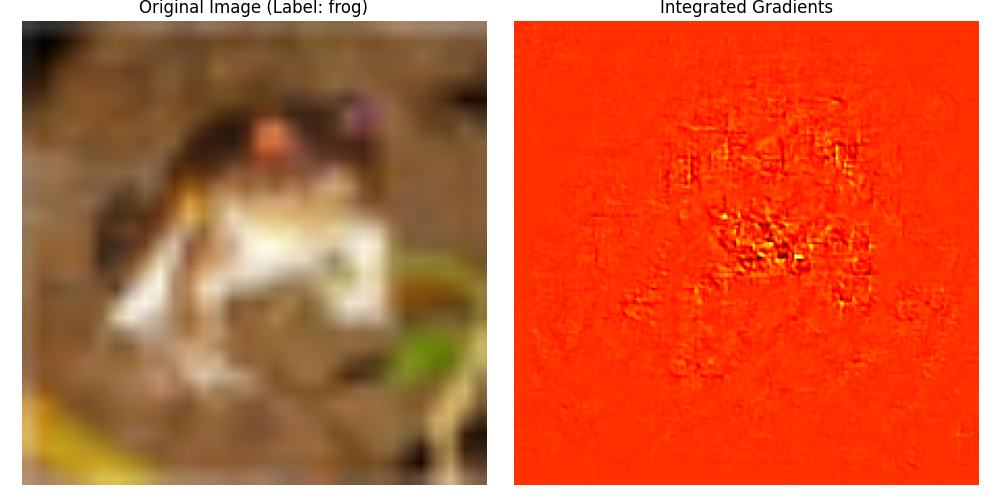
\includegraphics[width=0.5\textwidth]{images/integrated_gradients.png}
        \caption{Integrated Gradients zur Modellinterpretation}
  \end{figure}
\end{frame}

\begin{frame}{Erklärung für Sentiment-Analyse mit LLM}
  \begin{columns}
    \begin{column}{0.6\textwidth}
      \begin{itemize}
        \item \textbf{Ziel:} Generierung und Speicherung einer Erklärung für eine Sentiment-Analyse-Aufgabe.
        \item \textbf{Vorgehen:}
        \begin{itemize}
          \item Verwendung eines vortrainierten Sprachmodells (LLM) aus der Hugging Face Transformers-Bibliothek.
          \item Durchführung der Sentiment-Analyse auf einem Beispieltext.
          \item Visualisierung der Erklärung (z.B. Token-Wichtigkeit) als Balkendiagramm.
        \end{itemize}
        \item \textbf{Ergebnis:} 
        \begin{itemize}
          \item Die Bedeutung einzelner Tokens wird grafisch dargestellt, um die Entscheidungsfindung des Modells zu verdeutlichen.
        \end{itemize}
      \end{itemize}
    \end{column}
    \begin{column}{0.4\textwidth}
      \begin{figure}
        \centering
        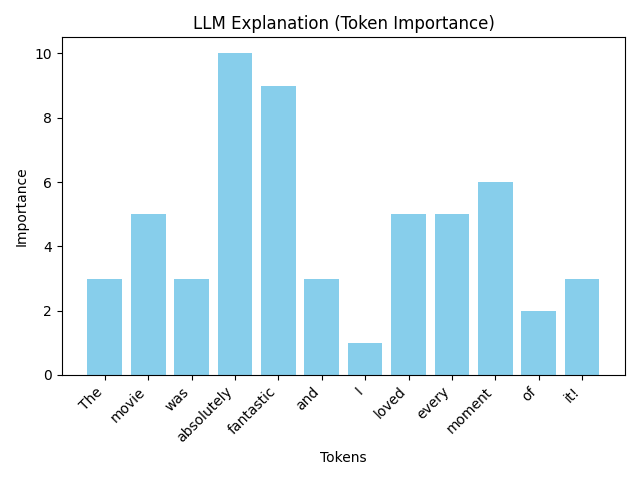
\includegraphics[width=\textwidth]{images/sentiment_explanation.png}
        \caption{Visualisierung der Token-Wichtigkeit für Sentiment-Analyse}
      \end{figure}
    \end{column}
  \end{columns}
\end{frame}

\begin{frame}{Interpretation von LLMs (Large Language Models)}
  \begin{itemize}
    \item \textbf{Herausforderungen:}
    \begin{itemize}
      \item Hohe Komplexität und Anzahl der Parameter erschweren die Nachvollziehbarkeit.
      \item Entscheidungen basieren auf nichtlinearen Beziehungen zwischen Tokens.
    \end{itemize}
    \item \textbf{Ansätze zur Interpretation:}
    \begin{itemize}
      \item \textbf{Attention Visualisierung:}
      \begin{itemize}
        \item Darstellung der Aufmerksamkeit (Attention Scores) zwischen Tokens.
        \item Tool: BertViz.
      \end{itemize}
      \item \textbf{Feature Attribution:}
      \begin{itemize}
        \item Identifikation der wichtigsten Tokens für eine Vorhersage.
        \item Tools: Captum, SHAP.
      \end{itemize}
      \item \textbf{Neuronale Aktivierungen:}
      \begin{itemize}
        \item Analyse der Aktivierungsmuster einzelner Neuronen.
        \item Tool: Neuroscope.
      \end{itemize}
    \end{itemize}
  \end{itemize}
\end{frame}

\begin{frame}{Bibliotheken zur Interpretation von LLMs}
  \begin{itemize}
    \item \textbf{BertViz:}
    \begin{itemize}
      \item Visualisierung der Attention-Matrizen in Transformer-Modellen.
      \item Unterstützt Modelle wie BERT, GPT-2.
      \item \url{https://github.com/jessevig/bertviz}
    \end{itemize}
    \item \textbf{Transformers Interpret:}
    \begin{itemize}
      \item Feature-Attribution-Methoden für Hugging Face Modelle.
      \item Unterstützt LIME, Integrated Gradients.
      \item \url{https://github.com/cdpierse/transformers-interpret}
    \end{itemize}
    \item \textbf{Captum:}
    \begin{itemize}
      \item PyTorch-Bibliothek für Interpretierbarkeit.
      \item Unterstützt Integrated Gradients, Layer Conductance.
      \item \url{https://captum.ai/}
    \end{itemize}
    \item \textbf{SHAP:}
    \begin{itemize}
      \item Shapley-Werte für Feature Attribution.
      \item Unterstützt Transformer-Modelle.
      \item \url{https://github.com/slundberg/shap}
    \end{itemize}
  \end{itemize}
\end{frame}
% ==================== XAI SECTION ====================
\section{Explainable AI weitere Quellen}

\begin{frame}{XAI Standardwerke}
  \begin{itemize}
    \item \textbf{Interpretable ML Book} (Molnar)
    \begin{itemize}
      \item \url{https://christophm.github.io/interpretable-ml-book/}
      \item Umfassender Leitfaden zu SHAP, LIME, etc.
    \end{itemize}
    \item \textbf{Explainable AI} (Springer 2019)
    \begin{itemize}
      \item DOI: \href{https://doi.org/10.1007/978-3-030-28954-6}{10.1007/978-3-030-28954-6}
      \item Forschungsbeiträge zu Deep Learning Interpretability
    \end{itemize}
  \end{itemize}
\end{frame}

\begin{frame}{XAI Toolkits \& Frameworks}
  \begin{itemize}
    \item \textbf{Quantus}
    \begin{itemize}
      \item \url{https://github.com/understandable-machine-intelligence-lab/Quantus}
      \item 35+ Metriken für XAI-Evaluation
      \item JMLR Paper: \href{https://www.jmlr.org/papers/v24/22-0142.html}{Quantus Paper}
    \end{itemize}
    \item \textbf{SHAP}
    \begin{itemize}
      \item \url{https://github.com/slundberg/shap}
      \item Shapley Values für Feature Importance
    \end{itemize}
    \item \textbf{AI Explainability 360} (IBM)
    \begin{itemize}
      \item \url{https://aix360.mybluemix.net/}
      \item Enthält ProtoDash, CEM
    \end{itemize}
  \end{itemize}
\end{frame}

\begin{frame}{XAI Forschungsarbeiten}
  \begin{itemize}
    \item \textbf{"Explainable AI: A Review"} (Gilpin 2018)
    \begin{itemize}
      \item \url{https://arxiv.org/abs/1801.00631}
      \item Systematische Klassifikation
    \end{itemize}
    \item \textbf{LIME Paper} (Ribeiro 2016)
    \begin{itemize}
      \item \url{https://arxiv.org/abs/1602.04938}
      \item Lokale Erklärbarkeit
    \end{itemize}
    \item \textbf{"Sanity Checks Revisited"} (Hedström 2023)
    \begin{itemize}
      \item Verbesserte MPRT-Metriken
    \end{itemize}
  \end{itemize}
\end{frame}

\begin{frame}[allowframebreaks]{References}
  \bibliographystyle{ieeetr}
  \bibliography{lit.bib}
\end{frame}
\end{document}
